\documentclass{article}
\usepackage[utf8]{inputenc}
\usepackage{amsmath}
\usepackage{graphicx}
\usepackage[procnames]{listings}
\usepackage{color}
\usepackage{indentfirst}
\usepackage{xcolor}
\usepackage{sectsty}
\usepackage[explicit]{titlesec}
\usepackage[normalem]{ulem}
\usepackage[hidelinks]{hyperref}
\title{Library Information System}

\author{}
\date{}


\begin{document}

\maketitle

\newpage
%\clearpage
\hypertarget{toc}{}
\tableofcontents


\section{INTRODUCTION}

\subsection{Purpose}
This Software Requirement Specification (SRS) document provides a complete list and description of all the functions and specifications of the Library Information System (LIS).

The software is meant to hold the records of the books and the users and to provide the functionality of issuing and returning books. Apart from that the users can also request to reserve a required book if available in the library.

The expected audience of this document are Library clerk , librarian of an institute and the developer of the software.
\subsubsection*{Problem Statement}
Different activities of the library of our institute pertaining to the issue and return of the books by the members
of the library and various queries regarding books as listed below are to be automated.
\begin{itemize}


\item The library has 10,000 books. Each book is assigned a unique identification number (called ISBN number).
The Library clerk should be able to enter the details of the book into the LIS through a suitable interface.
\item There are four categories of members of the library: undergraduate students, post graduate students,
research scholars, and faculty members.
\item Each library member is assigned a unique library membership code number.
\item Each undergraduate student can issue up to 2 books for 1 month duration.
\item Each postgraduate student can issue up to 4 books for 1 month duration.
\item Each research scholar can issue up to 6 books for 3 months duration.
\item Each faculty member can issue up to 10 books for six months duration.
\item The LIS should answer user queries regarding whether a particular book is available. If a book is available,
LIS should display the rack number in which the book is available and the number of copies available.
\item LIS registers each book issued to a member. When a member returns a book, LIS deletes the book from
the member’s account and makes the book available for future issue.
\item Members should be allowed to reserve books which have been issued out. When such a reserved book is
returned, LIS should print a slip for the concerned member to get the book issued and should disallow
issue of the book to any other member for a period of seven days or until the member who has reserved
the books gets it issued.
\item When a member returns a book, LIS prints a bill for the penalty charge for overdue books. LIS calculates
the penalty charge by multiplying the number of days the book is overdue by the penalty rate.
\item LIS prints reminder messages for the members against whom books are over due, upon a request by the
Librarian.
\item LIS should allow the Librarian to create and delete member records.
\item The Librarian periodically needs to check if there are any books which have not been issued even once
during the last five years. He uses this information in planning to dispose off unused and old books. For
this purpose it is necessary for LIS to maintain the statistics regarding issuance of different books.
\item When books are disposed off, the Library clerk should be able to delete the book from the list of books
in the Library and when a book is procured the system should support entering the details.
\end{itemize}
\subsection{Document Conventions}
The conventions used in the document are as per the IEEE standard provided for formatting the SRS document of a software

\subsection{Definitions}
The following terms are used in this document to refer to various componensts of the system :\\
%\begin{center}

\begin{tabular}{ c| c }
 Librarian & Person-in-charge (human administrator) of the software\\
 Member & Members of the library who can issue a book\\
 Issue & The act of borrowing a book by a user against his/her account\\
 Return & The act of returning the book issued by an user previously \\
 Reserve & The act of reserving a book currently unavailabele but for issuing in future\\
 Fine & The penalty to be paid by a user in case he/she fails the deadline to return the book\\
 ISBN & International Standard Book Number, a unique ID for each book
\end{tabular}	
%\end{center}

\subsection{Intended Audience}
The intended readers of this document are the developers of the software, testers, library owners
and managers and coordinators.\\
These people are meant to understand the details of the software architecture modelled and used to understand the proper functioning of the software and their individual roles in the software also.\\
Any suggested changes on the requirements listed on this document should be included in
the last version of it so it can be a reference to developing and validating teams.
\subsection{Scope}
LIS is a GUI tool that enhances the manual process of keeping records in a library.This is an appication which has been designed keeping in mind that it is meant to run on Library computers and to allow the library to keep a track of the books present.It allows the users to check availabilty whenever they want. It also allows the users to reserve a book in advance if needed. The librarian is able to keep a record of the overdue books, add new books, dispose old data, add new member or delete a member. 
\\
It is a powerful but still functionally simple library management software for big libraries and can provide a free easy-to-use system for rising libraries.
\\
Presently the maximum number of books has been kept constant to ensure a fruitful implementation of the software architecture. In future the list of books may be made to increase dynamically to make it more realistic.
\\
Also since the software is very useful and lightweight in design it may be further incorporated in a bigger software like school automation system or an university automation system of which this will be a small but a necessary module.
\\
The software may be futher modified to make a web interface also later in order to enable a remote access feature thus generalizing it further for common use of the public.
\subsection{References}
The following references have been consulted to make a suitable and effective software for library information system.

\begin{itemize}
\item IEEE standard 830-1998 recommended practice for Software Requirements Specifications-Description
\item 
\end{itemize}


\section{OVERALL DESCRIPTION}
\subsection{Product Perspective}
The product is meant to automate the manual work of a librarian and library clerk to increase the efficiency of the process. It will facilitate the users to check a book's availability status . One can reserve, issue and return a book via this software. The software is designed to automatically update the details in the account of the user thus minimizing the laboriuos work earlier used to be performed by the clerks in the manual process.
\\
One can genrate the reports and penalty bills via this software directly. It is designed to make the proces of issuing and searching books more easy.
\\
It is designed to make the process of issuing, reserving and returning of a book more swift and efficient with minimum manual effort.The background cron job takes care of updation of the user account in case any of the above functions are performed.

\subsection{Product Features}
The product provides the features to create a librarian , library clerks and a set of users comprising of UG student, PG student, Faculty and Research Scholar.

All the users irrespective of their type can issue and return a book.The librarian has some special functions like creation of a library member/user. The librarian can have access to account of any user and can look into it in case need arises.
Library clerks on the other hand can add and remove a book from the database of the library. They also have been assigned methods to impose fine in case of defautlters.

Finally there is a non-physical member called as LIS (syatem admin) which is autonomous and monitors all the finctioning of the software. It automatically notifies about the delays to the clerks and helps to update and keep track of all the activities of the software.

A class diagram showing the relationship is given below to enhance the understanding of the workflow.

subsubsection{Use cases}
\begin{enumerate}
\item User use cases:
	\begin{itemize}
	
	\item Query about Book\\
	\begin{itemize}
	\item Preconditions:\\
	1. The user must be logged in .\\
	2.The book must exist in the library\\
\item  Postcondition: \\If the book exists in the library,the availablity status of the book is returned\\
 \item Failure Situations:\\ The library does not have  the book \\
 \item Postcondition in case of failure:\\A message to user about the same\\
\item  Actors:\\ User communiates with the system\\
\item  Trigger:\\ User chooses the option to search books\\
 \item Main Success Scenario: \\The library has a copy of the book and it is available for issue.\\
\item  Extensions/Variations: \\The library has a copy of the book but currently none of the copies are available.The book maybe reserved by the user.
	\end{itemize}
 \item Issue Book\\
	\begin{itemize}
	 \item Preconditions:\\
	 1. The user must be logged in .\\
	 2.The book must exist in the library \\
	 3.It must be available for issue.\\
	 4.The user must not have exhausted his quota of number of books\\
 \item Postcondition:\\After successful issue the user account is updated\\
 \item Failure Situations:\\
 1. The library does not have  the book\\ 
 2.The library has the book and it is not avaiable for issue.\\
 3.The user has exhausted his quota of maximum number of books\\
 \item Postcondition in case of failure:\\In failure case 2. the user may choose to reserve the book if he has not exhausted his quota\\
 \item Actors:\\ User communiates with the system\\
 \item Trigger: \\User chooses the option to issue books\\
 \item Main Success Scenario:\\ The library has a copy of the book and it is available for issue.
	\end{itemize}
 

 \item Return Book\\
 \begin{itemize}
 \item Precondition:\\
 1.User must be logged in.\\
 2.User must have previously issued the book.\\
 \item Postcondition:\\
 1.If the book was overdue the penalty is calculated and a bill is printed\\ 
 2.In case the book was reserved by some other user, a notification is sent out to the other user.\\
 3.The user account is updated\\
 \item Failure Situations:\\The user has not issued any book\\
 \item Postcondition in case of failure:\\A message is give to the user about the same\\
 \item Actors:\\ User communiates with the system\\
 \item Trigger:\\ User chooses the option to return issued books\\
\item  Main Success Scenario: \\The user had previously issued the book\\
 \end{itemize}
 
 \item Reserve Book\\
	\begin{itemize}
	\item  Preconditions:\\
	1. The user must be logged in .\\
	2.The book must exist in the library\\ 
	3.It must not  be available for issue.\\
	4.The user must not have exhausted his quota of number of books\\
 \item Postcondition:\\
 1.After successful issue the user account is updated \\
 2.When the book is returned a notification is sent to the user.\\
 \item Failure Situations:\\
 1. The library does not have  the book \\
 2.The library has the book and it is  avaiable for issue.\\
 3.The user has exhausted his quota of maximm number of books\\
 \item Postcondition in case of failure:\\In failure case 2. the user may choose to issue the book if he has not exhausted his quota\\
 \item Actors:\\ User communiates with the system\\
 \item Trigger:\\ User chooses the option to reserve book\\
 \item Main Success Scenario:\\ The library has a copy of the book and it is not available for issue.\\
 
	\end{itemize}
 
 \item Cancel Reservation\\
 \begin{itemize}
 \item  Preconditions:\\
 1. The user must be logged in .\\
 2.The user must have reserved the book\\
 \item Postcondition:\\
 1.After successful issue the user account is updated \\
Failure Situations:\\The user has not issued any book\\
 \item Actors: \\User communiates with the system\\
 \item Trigger:\\ 
 1.User chooses the option to cancel reservation of a book \\
 2.User does not issue the reserved book within 7 days of return\\
 \item Main Success Scenario:\\ The library has a copy of the book and the user must have reserved it previously\\
	
 \end{itemize}

\item Pay Fine\\
	\begin{itemize}
	\item  Precondition:\\
	\begin{enumerate}	
	\item User must be logged in.\\
	\item User must have previously issued the book.\\The book must be overdue\\
	\end{enumerate}
 \item Postcondition:\\
  The book was overdue the penalty is calculated and a bill is printed 
 \item Failure Situations:
 \begin{enumerate}
 \item The user has not issued any book
  \item No returned books are overdue
	\end{enumerate} 
 \item Actors: User communiates with the system
 \item Trigger: User chooses the option to return issued books
 \item Main Success Scenario: The user had previously issued the book and the book is overdue
	\end{itemize}
\end{itemize}


\item Library Clerk Use Cases
 \begin{itemize}
 \item Enter details of a book
 \begin{itemize}
 \item Preconditions:1. The clerk must be logged in.\\2.The book must not be previously entered in the system
 \item Failure Situations:\\ The book is already in the system
 \item Postcondition in case of failure:\\A message to clerk about the same
 \item Actors:\\ library clerk communicates with the system
 \item Trigger:\\ Clerk chooses the option to enter new books
 \item Main Success Scenario:\\ The library  does not have the book and the book is newly entered in the system
\item  Extensions/Variations:\\ The library hasthe book and the umber of copies is increased
\end{itemize}
 \item Delete a book 
 \begin{itemize}
	\item 	Preconditions:\\1. The clerk must be logged in.\\2.The book must  be previously entered in the system \\3.The librarian has decided to dispose the book\\
 \item Failure Situations:\\ The book is not in the system\\
 \item Postcondition in case of failure:\\A message to clerk about the same\\
 \item Actors:\\ library clerk communicates with the system\\
 \item Trigger:\\ Clerk chooses the option to delete books\\
 \item Main Success Scenario:\\ The library  has the book and it is removed from the system.\\
 \item Extensions/Variations: \\The library has the book and the number of copies is reduced.\\
 
\end{itemize}	 
 
 \end{itemize}
 


\item Librarian Use Cases:
\begin{itemize}
 \item Add new member
 \begin{itemize}
  \item Preconditions:1.Librarian must be logged in\\2. A person must apply for membership
 \\ \item Postcondition:\\A new member account is created \\
 \item Failure Situations:\\ The user is already registered\\
 \item Postcondition in case of failure:\\A message to librarian about the same\\
\item  Actors:\\ Librarian communicates with the system\\
 \item Trigger: \\Librarian  chooses the option to add member\\
 \item Main Success Scenario:\\ The user is not previously registered\\
 \end{itemize}

\item Delete member\\ 
 \begin{itemize}
  \item Preconditions:\\ 1.Librarian must be logged in\\ 2. A person must apply for cacellation membership\\ 
 \item Postcondition:\\ The member account is deleted\\ 
 \item Failure Situations: \\ The user has no account\\ 
 \item Postcondition in case of failure:\\ A message to librarian about the same\\ 
 \item Actors: \\ Librarian communicates with the system\\ 
 \item Trigger:\\  Librarian  chooses the option to delete member\\ 
 \item Main Success Scenario:\\  The user   previously has an account\\ 
 \end{itemize}
 
 \item Order to print reminder\\ 
 \begin{itemize}
  \item Preconditions:\\ 1.Librarian must be logged in\\ 2. A book issued by a member must be overdue\\ 
 \item Postcondition:\\ A message is sent to the user.\\ 
 \item Failure Situations:\\  There are no overdue books\\ 
 \item Postcondition in case of failure:\\ A message to librarian about the same\\ 
 \item Actors: \\ Librarian communicates with the system\\ 
 \item Trigger:\\  Librarian  chooses the option to print reminder\\ 
 \item Main Success Scenario :\\  There are some overdue books\\ 
 \end{itemize}

\item Plan to dispose books\\ 
 \begin{itemize}
  \item Preconditions:\\ 1.Librarian must be logged in\\ 2. The book must not have been issued even once for 5 years\\ 
 \item Postcondition:\\ The book is disposed with a message to the library clerk to delete it.\\ 
 \item Actors:\\  Librarian communicates with the system\\ 
 \item Trigger:\\  Librarian  chooses the option to dispose book\\ 
 \item Main Success Scenario:\\  The book has not been issue for 5 years\\ 
 \end{itemize}
 

\end{itemize}

\item System Use Cases:\\ 
 \begin{itemize}
 
  \item Answer availibilty Query about Book\\ 
	\begin{itemize}
	\item  Preconditions:\\ 1.An user makes a query\\ 
 \item Postcondition: \\ If the book is available, use cases display rack number and number of copies are called\\ 
 \item Actors:\\  System communiates with the user\\ 
 \item Trigger: \\ User chooses the option to search books\\ 
	\end{itemize}

\item Display rack number of book\\ 
	\begin{itemize}
	\item  Preconditions:\\ 1.If the book is available the use case answer availibility query invokes this\\ 
 \item Postcondition:\\  Rack numbers are displayed\\ 
 \item Actors:\\  System communiates with the user\\ 
 \item Trigger:\\  answer availibity query triggers this\\ 
	\end{itemize}
 
 \item Display number of copies of book\\ 
	\begin{itemize}
	\item  Preconditions:\\ 1.If the book is available the use case answer availibility query invokes this\\ 
 \item Postcondition:\\  the number of copies of a book are displayed\\ 
 \item Actors: \\ System communiates with the user\\ 
 \item Trigger:\\  answer availibity query triggers this\\ 
	\end{itemize}

\item Calculate lateness penalty\\ 
	\begin{itemize}
	\item  Preconditions:\\ 1.If the book is overdue, return book invokes this\\ 
 \item Postcondition:\\ Penalty is calculated and print bill is invoked\\ 
 \item Actors: \\ System communiates with the user\\ 
 \item Trigger: \\ return book query triggers this\\ 
	\end{itemize}
 
 \item Provide book issue statistics
	\begin{itemize}
	\item  Preconditions:\\ 1.The use case is invoked by plan to dispose books\\ 
 \item Postcondition:\\ Statistics of books is displayed\\ 
 \item Actors: \\ system communicates with librarian\\ 
 \item Trigger:\\ Plan dispose book is invoked\\ 
	\end{itemize}

 \end{itemize}
\item Printer use cases:\\ 
\begin{itemize}
\item Print bill of penalty\\ 
\begin{itemize}
\item Preconditions:\\ Some user must have returned the issued book later than his designated return date.\\ 
 \item Postcondition:\\ Bill of penalty is printed\\ 
 \item Actors:\\  Printer communiates with the system\\ 
 \item Trigger:\\  Calculate lateness penalty triggers print bill\\ 
\end{itemize}

\item Print reminder\\ 
\begin{itemize}
\item  Preconditions:\\ Some user must have exceeded the due date\\ 
 \item Postcondition:\\ Reminder to user is printed\\ 
 \item Actors:\\  Printer communiates with the system\\ 
 \item Trigger:\\ order to print reminder triggers this\\ 
\end{itemize}

\item Print notification on return of reserved book\\ 
\begin{itemize}
\item Preconditions:\\ Some user must have returned a reserved book \\ 
 \item Postcondition:\\ A notification is printed to the user who reserved the book\\ 
 \item Actors: \\ Printer communiates with the system which communicates with user\\ 
 \item Trigger:\\ return book may trigger this use case\\ 
\end{itemize}

\end{itemize}
\end{enumerate}
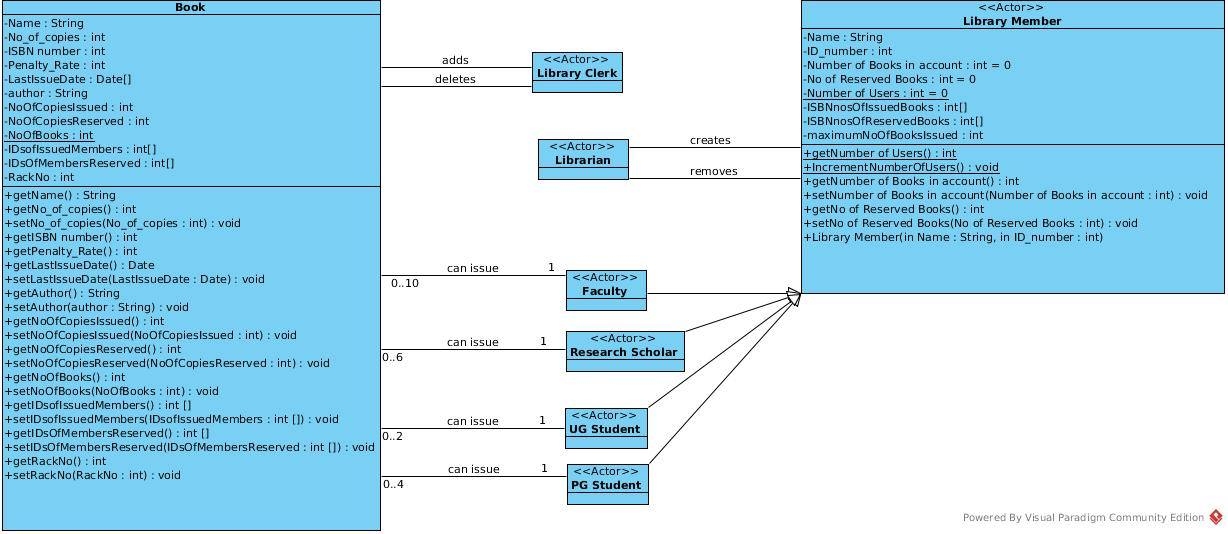
\includegraphics[scale=0.25]{images/classDiagram}
\\
%\begin{itemize}
%\item Issue Book : Allows the librarian to issue books to members on request
%\item Return book : Whenever a member returns an issued book , the library system uses this data to update the database and user history simultaneouly. This data can also be used to calculate fine if the book is returned late than the deadline
%\item Add book : It allows the librarian to add books to the library database
%\item Delete book : The librarian has an option to remove a book from the library database
%\item Add/Remove members : The software allows the user to add members like the faculty and the other students to have access to the books in the library
%\item View history : The librarian can view the issue history of any book in the library
%\item Query : The library can search for a particular book by giving a part of its name or the full name of the book.
%\end{itemize}

\subsection{User Classes and Characteristics}

\subsection{Operating Environment}
The software is designed to run on the following environments :
\begin{itemize}
\item Windows 
\item Ubuntu 14.04.03 (LTS version)

Any OS with the support of Java JDK and JRE libraries 1.7 and above can be used to execute the software.
\end{itemize}

\subsection{Design and Implementation Constraints}
This software is optimized to run on a maximum of 10000 books .
Exceeding this number can result in a slower running time of the algorithm and thus the execution may not fruitful enough.

\subsection{User Documentation}
User manual $:$

\subsubsection*{User Login}
Any user with a valid username and password will be able to login to the software to access the features. Initially just after the installation of the software only a librarian can be created in the software. Upon thd creation of the librarian the librarian can then create the other users in the library.
\begin{itemize}
\item For librarian : If a user logs in as librarian he is then shown a librarian home page screen with the functionalities exclusively of a libraraian.
\item For clerk : If user logs in as clerkhe is then shown the clerk home page with the functions like adding or deleting book etc.
\item For others(members) : We switch on to a new screen which is the home screen of the member. The member has the options of issuing, reserving and returning a book.
\end{itemize}

\subsubsection*{User creation}
The librarian can be created in the beginning when the software is first installed. Once a librarian is creates an new librarian can not be created until and unless the old one is removed.
\\
Only the librarian can create a new member of the library like the faculty or the students.
During the creation of a member the librarian should also provide the type of the user as the maximim book count is different for different categories of the users.Once the type of a library member is given during creation one does not need to provide it anywhere else during issuing or returning of a book as it will be saved in the database and automatically fetched when required.

\subsubsection*{Librarian Home Screen}
The librarian hold the administrator access of the library.The feature available to him are as follows :
\begin{itemize}
\item Creation of user :
For this purpose the librian will be directed to a new scree where he will have to provide the necessary details in order to create a new account and he has to provide the member type during account creation.
\end{itemize}

\subsection{Assumptions and Dependencies}


\section{SYSTEM FEATURES}
\subsection{User login}
The software should allow the user to provide the details of a user to login into the system.
\subsection{Add user}
The librarian is allowed to create a new user of the library who can have the facilities like issuing , searching and returning of a book.
\\
The librarian gives the valid details in the fields to make the user and adds it to the database
\subsection{Remove user}
The librarian who hold the administrator acces to the software can remove any user from the user if need arises.All the records of the user will be removed from the databse maintained in the software.
\subsection{Search book}
A library user(faculty,research scholar,UG or PG student) can search a book to see if it is available in the library for issuing.

\subsection{Issue book}
A library user(faculty,research scholar,UG or PG student) can issue a book which is available in the library only if he/she has not exceeded the maximum issue count aginst his/her account.
\subsection{Return book}
A library user(faculty,research scholar,UG or PG student) can return a book which is available in the library only and is liable to pay fines in case of overdue.

\subsection{Give penalty}
A library user(faculty,research scholar,UG or PG student) can pay the fine if he/she has aprevious overdue dute to late returning of a book.


\section{EXTERNAL INTERAFCE REQUIREMENTS}
\subsection{User Interfaces}
\subsection{Hardware Interfaces}
\begin{enumerate}
\item The software is run offline so hard disk with sufficient space of about --- is required to store and save the records for further use
\item Keyboard and mouse to interact with the GUI
\end{enumerate}
\subsection{Software Interfaces}
\begin{enumerate}
\item Back end  $:$ Built using Java and DBMS(MySQL)
\item Front end $:$ Using Java 
\end{enumerate}

\subsection{Communication Interfaces}
The databases can be kept in a separeate location other than the source computer itself to make it more space efficient.It can be done by using tcp/ip protocol for network access.It is not mandatory fot this specific design but can be taken up as a  feature which can be appiled to make the software more realistic and user friendly.

\section{OTHER NONFUNCTIONAL REQUIREMENTS}
\subsection{Performance Requirements}
With the Library Information System the librarian and library clerk can process a book transaction in a faster speed .
The members will be able to check the status of the checked out items and can also borrow and return a book in a short amount of time.
Automatic updates in the account of each user will enable them to know about the item they have checked out and all the relevant details due to which they do not need to consult or ask the library clerk each time.
The background system admin will automatically perform the above mentioned updation in the accounts in the background autonomously without explicit invocation.
In case of defaulters the fine and other penalties should be automatically reported and saved in the record once the deadline has crossed . This is also performed by the syatem admin (referred as LIS itself) in the background.
ALl the background tasks should not compromise with the UX of the software.All the background processes should be methodically handled and not affect the runtime functionalities of the software

\subsection{Safety Requirements}
Only the valid users can change the records that too only in their respective account.In case any invalid user tries to tamper with the data a error message will be flagged thus aborting the action.
\subsection{Security Requirements}
The sytem must be highly secure in the login part.
No user should be able to access a domain outside his reach.
Care must be taken to keep the user accounts secure and all the book transaction should be properly updated to the corresponding user.

\subsection{Software Quality Requirements}
\subsubsection{Reliability requirements}
The software is extremely reliable and has a lightweight design.It uses as minimum resources as possible but still it provides a quality support for the intended software requirements.
Multiple copies of the database have been kept at sepearte locations to ensure that the data is not lost in case of a serious software glitch. These backup datasets can be recovered easily by a file reader to get back the lost data.
\\
The background database should always be updated so that whenever a member visits he/she can get the latest information required.Also the duplicate or the backup databases must also be updated at the same time so that no discrepancy is there among the parallel databases.
\\
For every process that the software can do the steps are quite clearly framed and unambiguous in nature so that the user will not face any problem in doing the job.
\subsubsection{Usability Requirements}
The software must be user-friendly so that the user can easily perform all the tasks which the software is meant to do.It must have a soothing UX design and clear instructions to guide the user.
\\In case of any error suitable error messages must be displayed to assist the user.Also a user manual is provided with the glimpses of the software design to show how the softwar eis supposed to work.
\\
Care has been taken to make the software process very fast and reliable.The running time of the software and the space complexity have been optimized as far as possible to keep the software more realistic and usable


\section{OTHER REQUIREMENTS}
The other thing which is required to make the back-end of the software is sql support. The sql framework used behind this software is MySQL for JAVA. Using the packages the sql support has been estblished.\\
Use of sql is there to ensure proper database facilities rather than just using normal text files which might have also served our purpose.Use of proper databse structure greatly reduces the running time making it logarithmic from linear with respect to the number of records.
\\


\end{document}